\chapter{Introduction}
\lhead{\chaptername~\thechapter. \emph{Introduction}}
The growing interest of the general public in spherical cameras technologies, which were 
research-only exclusives once, has made them less expensive and more available. For example, omindirectional cameras by GoPro have been extremely popular amongst sports men who publish them on social networks.

These devices have been employed in robotics since their first appearance to help navigate the robot in a real-world environment, and nowadays for autonomous driving. Furthermore, they can be exploited to deliver a virtual or augmented experience for augmented and virtual reality (AR/VR).

In this work, we designed a \textit{structure from motion} (SfM) pipeline for 
full spherical cameras. SfM is a well known topic in computer vision; it addresses the problem of 
recovering the structure of 3D environments from a sequence of images taken from different views.

SfM research (and computer vision in general) has targeted perspective cameras because these type of devices have always been more common. However, the increase of interest around these cameras has started a shift of interest towards employing them for research.

\section{Omnidirection Cameras}
Large field of view (FOV) photography employs fisheye lenses that are capable to cover 
wider scene compared to traditional cameras' hardware.
The applications for this kind of equipments range from architectural or 
landscape photography to academic use for studies related to astronomic, 
meteorology, computer graphics, etc.
Photographers can also choose fisheye lenses for the characteristic distortion
these devices introduce and that provides more importance to foreground objects
(see Figure~\ref{fig:wide_fov_pics}~(\subref{fig:fisheye_example}) for an 
example of a picture taken with fisheye lenses equipped camera).
An example of wide FOV photography equipment is the GoPro\registered's camera series.
GoPro Inc\registered. produces action cameras, small digital devices for recording videos 
and taking pictures in harsh environments; their products have gained quite 
some success among the consumer market, also thanks to their marketing campaign 
that successfully associated their product to extreme sport events.
Action cameras like GoPro\registered's exploit wide FOV lenses that help to capture larger
scenes and make the devices fit to be worn.

Apart of wide FOV hardware there is another class of  
cameras that take panoramic photography to a new level: 
the 360\degree full spherical devices, capable of capturing images
in every directions with no blind sides. This class of devices employs 
several image sensors and integrated stitching software to automatically produce
panoramic pictures. This is the case for the Ricoh Theta S\texttrademark 
\cite{theta_website} we used in this work (Figure~\ref{fig:ricoh_theta}).

Together with consumer hardware, some off the shelf
solutions for the professional market have started to appear; they include the Insta360
Pro\registered that can capture full spherical videos or pictures
at 8K resolution.
The GoPro Omni\registered is an alternative to the previous, it is a simple 
rig that contains 6 traditional GoPro\registered devices and that comes with 
specialized software to enables the 360\degree videos 
creation.

The interest in full spherical media creation is driven by the introduction 
of  new immersive media fruition devices, like 
\textit{head-mounted display} (HMD) or mobile visors.
\begin{figure}
	\centering
	\begin{subfigure}{0.3\textwidth}
		\centering
		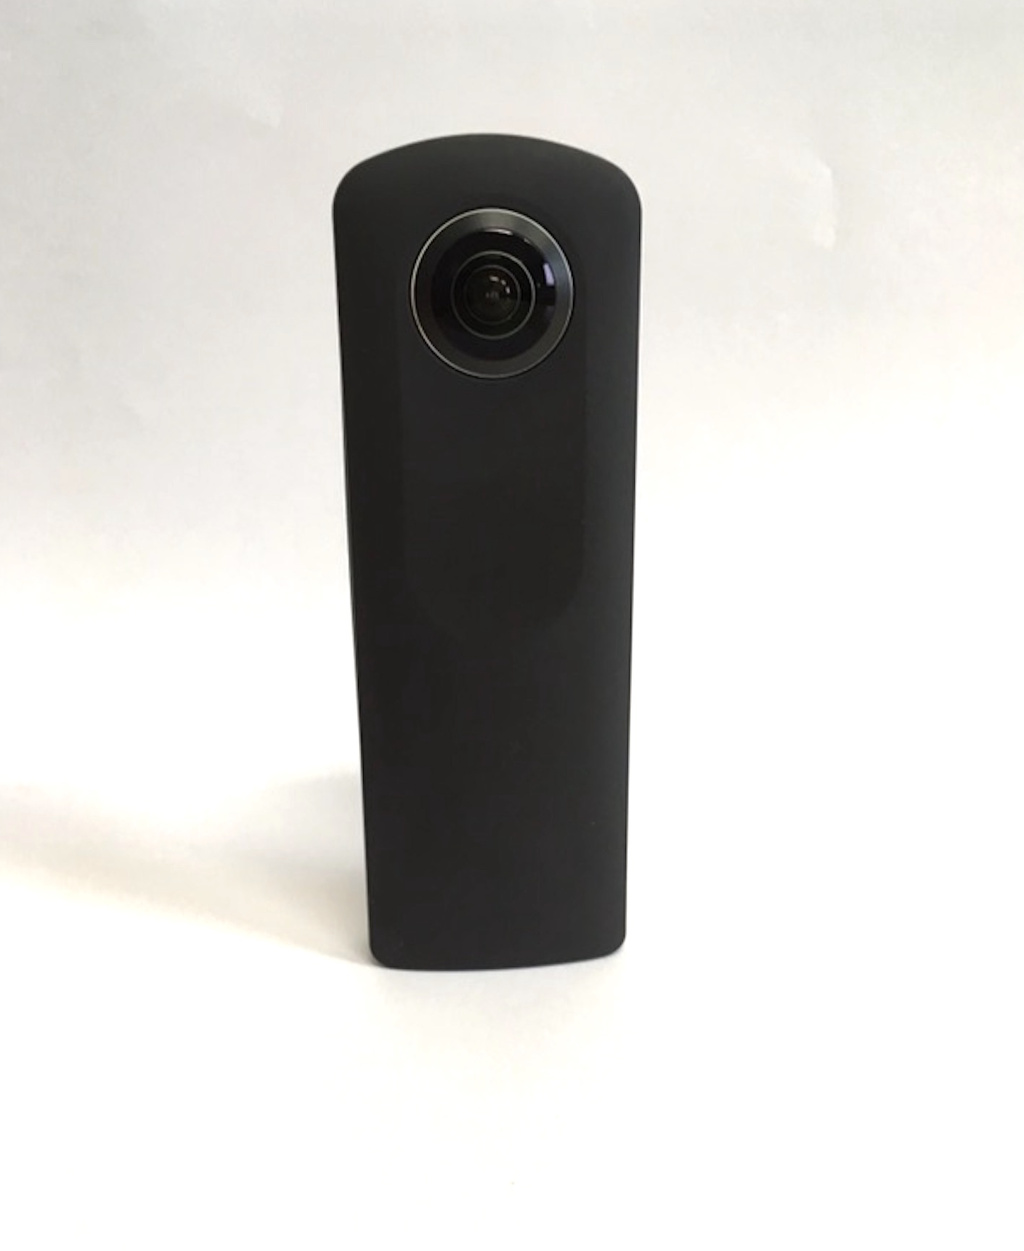
\includegraphics[width=0.7\textwidth]{img/theta1}
	\end{subfigure}
	\begin{subfigure}{0.3\textwidth}
		\centering
		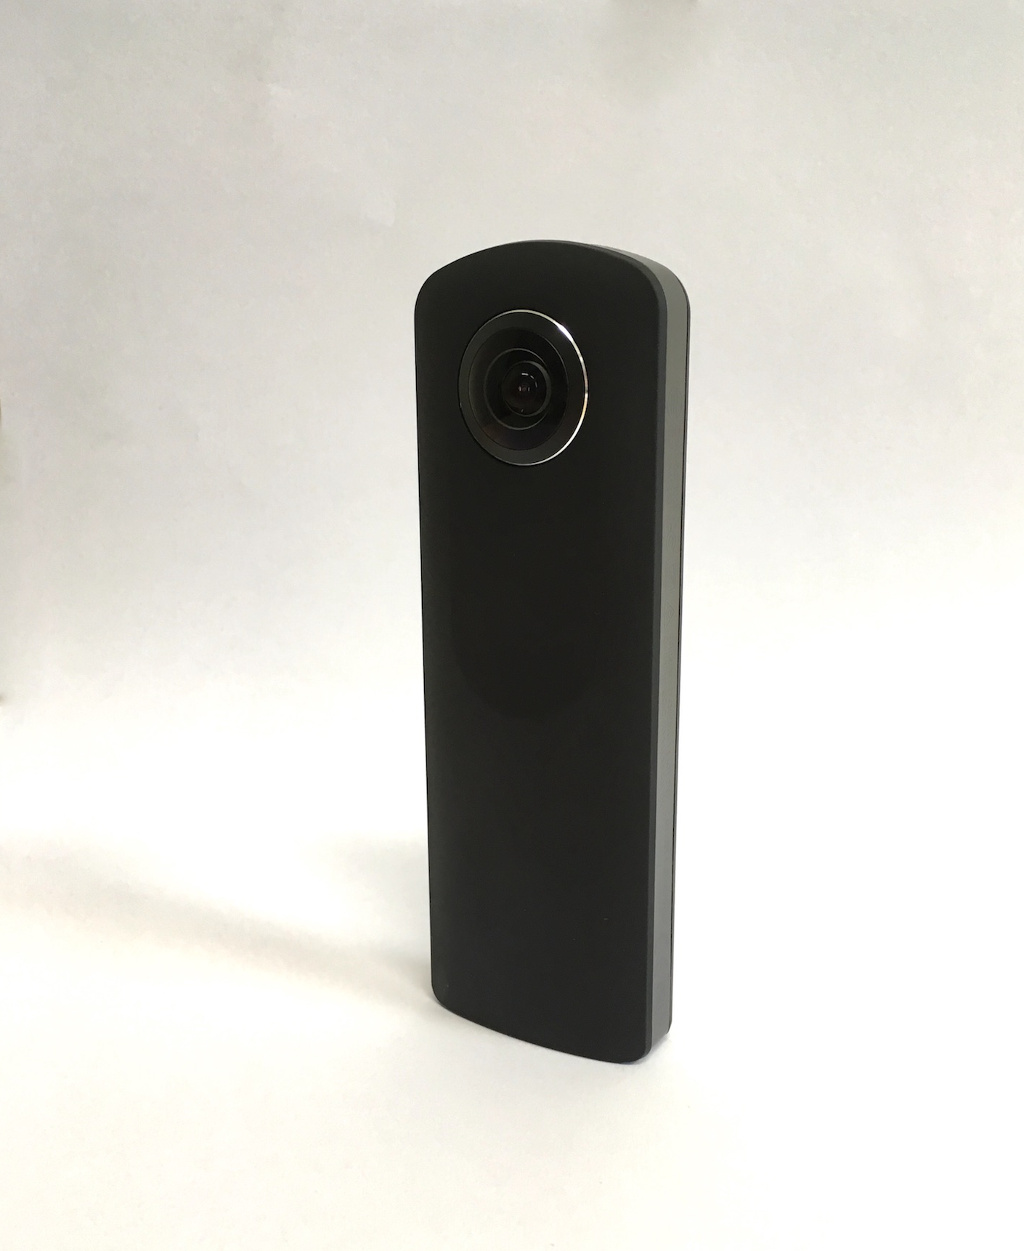
\includegraphics[width=0.7\textwidth]{img/theta2}
	\end{subfigure}
	\begin{subfigure}{0.3\textwidth}
		\centering
		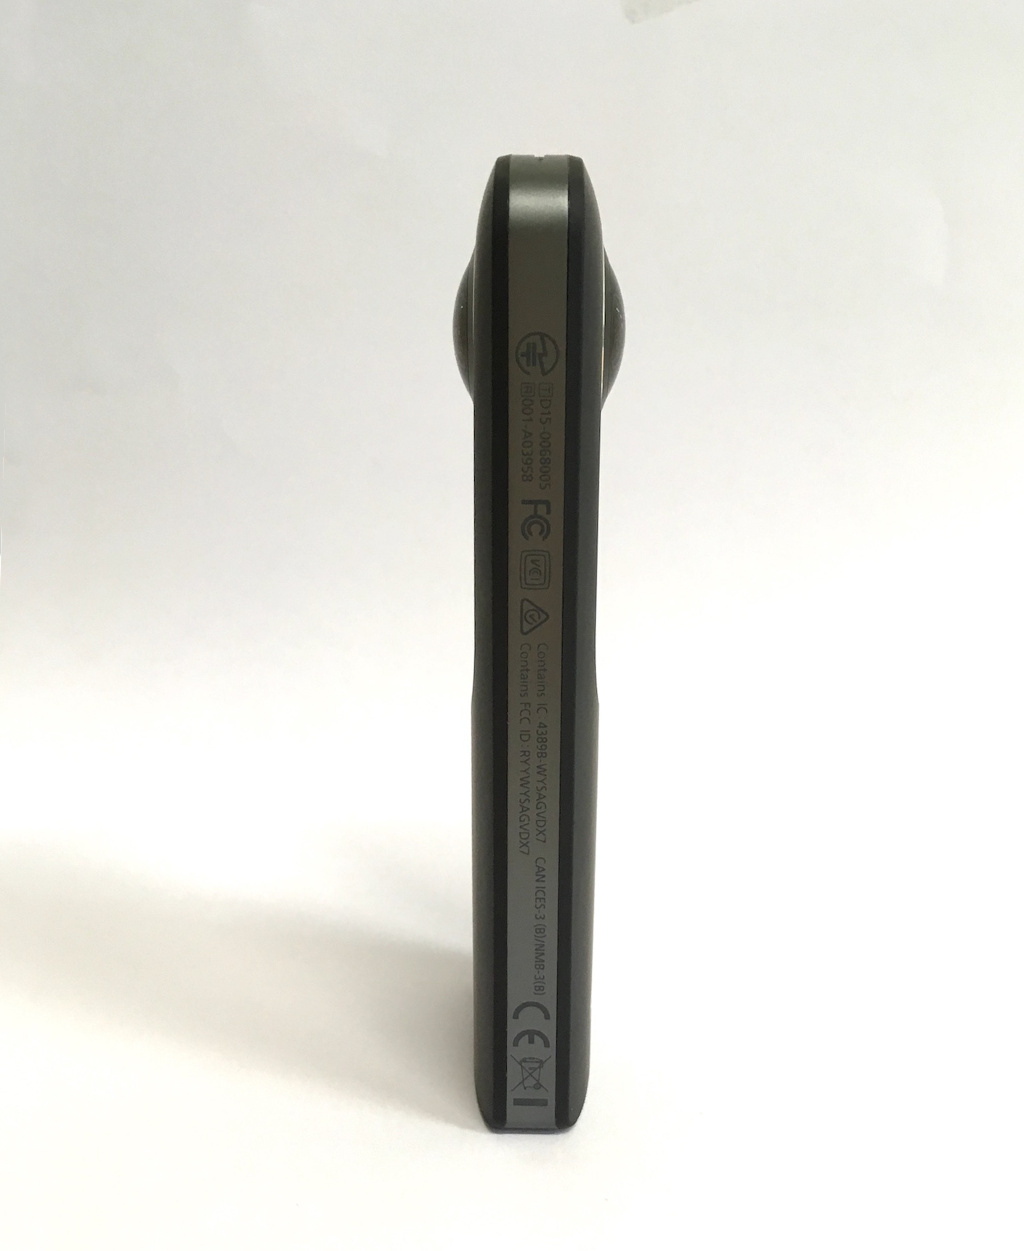
\includegraphics[width=0.7\textwidth]{img/theta3}
	\end{subfigure}
	\caption{\label{fig:ricoh_theta}The Ricoh Theta S 360\degree camera.}
\end{figure}

\begin{figure}
	\centering
	\begin{subfigure}{0.4\textwidth}
		\centering
		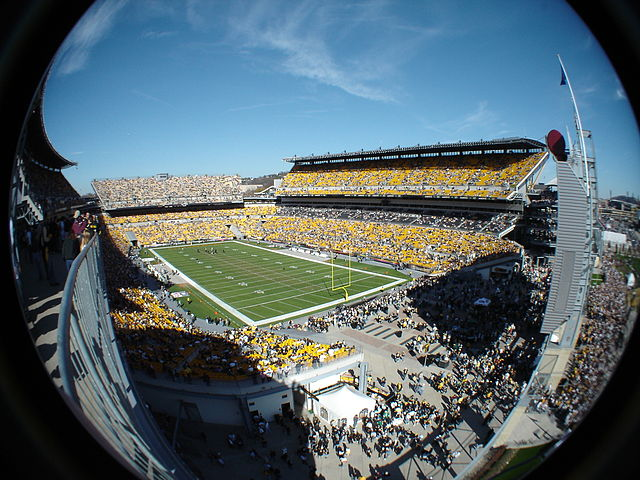
\includegraphics[width=0.7\textwidth]{img/fisheye_example}
		\caption{Fisheye.}\label{fig:fisheye_example}
	\end{subfigure}
	\begin{subfigure}{0.4\textwidth}
		\centering
		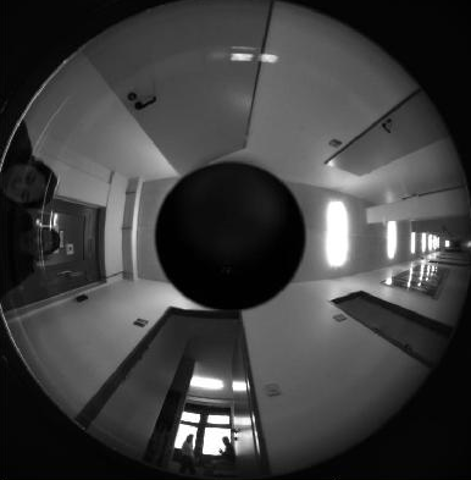
\includegraphics[width=0.7\textwidth]{img/omnidirectional_example}
		\caption{Ominidirectional (catadioptric).}\label{fig:omnidirectional_example}
	\end{subfigure}
	\caption{Some example of fisheye (\subref{fig:fisheye_example}) and omnidirectional (\subref{fig:omnidirectional_example}) pictures.}\label{fig:wide_fov_pics}
\end{figure}

\section{Benefits of Full Spherical Cameras}
Because of the increased \textit{field of view} (FoV), panoramic cameras can capture a larger amount of data compared to traditional devices. For example, the two fisheye lenses in the Ricoh Theta allow users to utilize also rear correspondences between images and this may improve the quality of motion estimation.

Another advantage of full spherical cameras is that they do not require a calibration phase for intrinsic parameters estimation. Camera calibration is an essential requirement for most computer vision applications, which estimates several parameters such as focal length, image 
sensor size, pixel density, and lens distortion model. When dealing with full spherical cameras, we can assume the image is taken from a unitary sphere. Therefore, we can set the focal length to 1. Further details about the camera model and the parameters can be found in Chapter~\ref{ch:state_of_the_art}.

\section{SfM Applications}
SfM is a well known topic in the computer vision community; it was born after 
the landmark paper by Longuet-Higgins \cite{longuet1981computer}, and
Nister et al. \cite{moravec1980obstacle}.
The problem can be described as the reverse of image formation
\cite{Wei2013}, as it targets the reconstruction of the environment 
and camera poses given a set of two or more images.
Some of the first application for this technology included robotic research, 
like navigation systems intended for rover explorations 
\cite{moravec1980obstacle,durrant1996localization}. In fact, NASA have supported
many researches because of the need for navigation systems not affected by wheels
slippage on uneven terrains.
SfM is used in geographical data acquisition too
\cite{fonstad2013topographic,westoby2012structure,james2012straightforward}
as alternative to other methods that employ specialized hardware and 
come to higher price.
There are also applications for cultural heritage conservation since 
environment reconstructions can help in case of restoration of historical finds
\cite{kraus2007photogrammetry}.
The game industry is yet another field that can benefit from 
SfM: real environments can be reconstructed with SfM first and then 
improved by artist. Some game engine, like the popular Unreal Engine\registered,
includes photogrammetry software that exploits SfM techniques. \todo{non ho trovato un riferimento}
\todo[inline]{chiedere per un esempio di foto fisheye}
